\chapter{Experiments} \label{sec:experiments}

This section aims to empirically test how effective subject-driven augmentation is in improving the performance of computer vision models. Our approach consists of testing how competitive this data augmentation technique is on real tasks compared to other well-known methods such as Autoaugment or RandAugment. In addition, we study the behaviour concerning the ratio of real images to synthetic images and check how much information can be obtained using only synthetic images. On the other hand, we test control techniques to try to improve the results. With these, we demonstrate whether the proposed augmentation approach can enhance the performance of segmentation models. Finally, we test in other domains to see if the process is generalisable to other datasets.

Our results support the hypothesis that subject-driven augmentation is a competitive data augmentation technique in real tasks. In particular, we show that it is especially significant when training data is sparse. Thus, we observe accuracy increases of up to 19.11\% in classification tasks using the Oxford-IIIT Pet dataset. However, we show that adding synthetic images to a small dataset only makes sense to a certain extent, especially when sufficient real training images are available. Furthermore, we show that competitive results can be obtained using only synthetic images in training a computer vision task. Finally, we demonstrate the versatility of this approach by showing its application in various tasks, including segmentation, as well as its potential on alternative datasets such as Food-101.

\section{Experiments overview} \label{sec:experimentsO}

The first step in testing the capabilities of subject-driven augmentation is to know the limitations of the selected subject-driven techniques. If we consider Dreambooth and Textual inversion, we will realise that their main input element is images of a specific subject. Two fundamental questions arise at this point. Firstly, how many images are to be used? Secondly, is it feasible to apply Dreambooth and Textual inversion to different subjects of the same class?

For this reason, we initially set up the experiment \textbf{01-number-of-images}. In this experiment, we want to test the effect of the number of images used in applying subject-driven generation techniques on the quality of the images generated. Dreambooth and Textual inversion authors propose using between 3 and 5 images \cite{ruiz2022dreambooth, gal2022image}. However, since the proposed pipeline will push these techniques to their limits by selecting images of subjects that do not necessarily have to be the same, it is interesting to see how flexible they are. Therefore, the \textit{01-number-of-images} experiment proposes to test 1, 2, 3 and 5 images. These tests allow the flexibility of Dreambooth and Textual inversion to be tested to establish an appropriate number of images.

On the other hand, the question remains whether it is feasible to push these methods to the limit with images of subjects that, although of the same class, are different. Thus, we define the experiment \textbf{02-different-subjects}. It aims to test how flexible Dreambooth and Textual inversion are when provided with several images of different subjects sharing the same class. To do so, we take the domain of dog breeds and employ subject-driven generation methods on sets of images that mix dog breeds. Furthermore, we perform the experiment incrementally to maximise the information we can extract from the performance of Dreambooth and Textual inversion. Initially, we take dogs with a common breed, and successively, we introduce dogs of increasingly different breeds. Specifically, we start with a Golden Retriever and successively add subjects of the following breeds: German Shepherd, Siberian Husky, Bulldog and Welsh Corgi.

At this point, the experiments \textit{01-number-of-images} and \textit{02-different-subjects} give us an insight into the possibilities of subject-driven generation techniques. Therefore, we can move on to experimenting with the entire pipeline. In experiment \textbf{003-training-percentage}, we intend to compare it with other data augmentation techniques. The selected task consists of classification on the Oxford-IIIT Pet dataset. The selected approaches are as follows.

\begin{itemize}
    \item \textbf{Baseline}: Common and comparative starting point for assessing the performance of other approaches. It helps to establish the minimum expected level of performance. It is the vanilla classification task, i.e. without additional data augmentation or modification.
    \item \textbf{Custom data augmentation}: The training set is extended with classical transformations such as horizontal flips, rotations, and brightness and contrast adjustments, among others.
    \item \textbf{AutoAugment}: An automated augmentation policy developed by Google Brain \cite{cubuk2018autoaugment} is used for data augmentation.
    \item \textbf{RandAungment}: An improved automated augmentation policy developed by Google Brain \cite{cubuk2020randaugment} is used for data augmentation.
    \item \textbf{Dreambooth}: The subject-driven augmentation pipeline based on Dreambooth is used, as described in section \ref{sec: sdAugmentation}. 
    \item \textbf{Textual inversion}: The subject-driven augmentation pipeline based on Textual inversion, as described in section \ref{sec: sdAugmentation}, is used.
    \item \textbf{Stable Diffusion prompt}: The subject-driven augmentation pipeline based on class names, as described in section \ref{sec: sdAugmentation}, is used.
\end{itemize}

However, experiment \textit{03-training-percentage} continues beyond there and compares these approaches by varying the percentage of real data used in the training set. In this way, we can check what effect the size of the dataset has on the effectiveness of one or the other technique. Finally, it is important to highlight that subject-driven approaches use 50 synthetic images. However, for specific implementation details, please refer to section \ref{sec: implemantationD}.

Once it is known how the selected techniques perform when the size of the training set is varied, it is logical to think that the next step is to vary the number of images generated. Along these lines, in the \textbf{004-generation-percentage experiment}, we vary the percentage of images generated while leaving the size of the actual training set fixed. In this way, we can test how many synthetic images perform better with respect to the accuracy of the task.

After completing experiments \textit{03-training-percentage} and \textit{04-generation-percentage}, to what extent are real images necessary to obtain competitive results? To address this question, we set up experiment \textbf{005-all-generated}. In it, we only train the classification model with synthetic images, and the objective is to determine the quality of the information in the images. That is, to what extent can the text-to-image model generate images with valid information that a classification model can subsequently extract? In this way, it can be considered a case of transfer learning in which a larger model transfers information to a smaller model. In this case, through images.

However, the approach projected in the \textit{05-all-generated} experiment has a fundamental problem. Dreambooth and Textual inversion need real images as inputs. Therefore, the premise of not using any real images is not being fulfilled. However, the Stable Diffusion prompt approach (based on generating images using only class names, figure \ref{fig:controlNetP}) does not require any input images. Therefore, its results are valid.

Experiment \textbf{06-controlnet} adds conditional control to the images generated by the Stable Diffusion prompt approach. Figure \ref{fig:controlNetPipe} shows the pipeline used. Its purpose is to test whether the quality of the synthetic images can be improved by adding control.

Another interesting question is whether classical data augmentation techniques are capable of being used in combination with the subject-driven approach. Thus, the \textbf{07-combinations} experiment seeks to merge the best subject-driven configurations found with classical techniques such as RandAugment. The combination could improve the results of both techniques separately. 

So far, we have only considered a classification task on the Oxford-IIIT Pet dataset. Thus, the \textbf{08-segmentation} experiment moves the subject-driven approach to a segmentation task on the same dataset. It employs conditional control, as does experiment 06-controlnet. On the other hand, experiment \textbf{09-food-101} seeks to test another dataset to demonstrate the versatility of subject-driven augmentation.

In summary, we conducted the following experiments in this paper to learn about the strengths and weaknesses of subject-driven augmentations.

\begin{itemize}
    \item \textbf{01-number-of-images}: It takes Dreambooth and Textual inversion to study the effect of the number of real images used as input. This is interesting as it allows us to explore the limits of these techniques. This is essential since the proposed augmentation pipeline requires these methods to provide great flexibility.
    \item \textbf{02-different-subjects}: The objective is to examine whether it is feasible to push these methods to the limit with images of subjects that, although of the same class, are different. Thus, we take the domain of dog breeds and employ subject-driven generation methods on sets of images that mix dog breeds incrementally by considering less and less similar breeds.
    \item \textbf{03-training-percentage}: This experiment goes on to test the entire pipeline. In this way, we intend to compare it with other data augmentation techniques. Specifically, we define tests with a baseline, classical data augmentation techniques, automated augmentation policies such as AutoAugment and RandAugment, and the subject-driven augmentation pipeline defined with Dreambooth, Textual inversion and Stable Diffusion prompt. In addition, this experiment compares these same approaches by varying the percentage of real data used in the training set. The number of synthetic images is set to 50.
    \item \textbf{04-generation-percentage}: It takes 03-training-percentage and varies the percentage of images generated while leaving the size of the actual training set fixed.
    \item \textbf{05-all-generated}: The purpose is to evaluate whether a computer vision model can only be trained with synthetic images and obtain competitive results. However, it should be noted that both Dreambooth and Textual inversion need real images to personalise the text-to-image model. Therefore, their results should be interpreted with caution. However, the Stable Diffusion prompt approach can be run with no real images, only with class names.
    \item \textbf{06-controlnet}: It aims to test whether the quality of synthetic images can be improved by adding conditional control. It considers the Stable Diffusion prompt approach. 
    \item \textbf{07-combinations}: It merges the best subject-driven configurations found with classical techniques such as RandAugment. The idea is that the combination could improve the results of both techniques separately.
    \item \textbf{08-segmentation}: Moves the subject-driven approach to a segmentation task. 
    \item \textbf{09-food-101}: Considering an utterly different dataset, it aims to see how versatile subject-driven augmentation is.
\end{itemize}

\section{Implementation details} \label{sec: implemantationD}

Next, the aspects of the code implementation carried out to execute the experiments defined in \ref{sec:experimentsO} are detailed. Thus, the details concerning the datasets, the neural networks, the subject-driven techniques and the hardware and execution environment are explained. The aim is to make the detailed analysis in this work as rigorous and thorough as possible. And, consequently, to allow replicability so anyone can certify the results obtained.

\subsection{Datasets}

The primary dataset chosen for the present work is Oxford-IIIT Pet \cite{Parkhi2012CatsAD}, a collection of 7,349 images of cats and dogs of 37 different breeds, of which 25 are dogs, and 12 are cats. The dataset contains about 200 images for each breed. We divide these images randomly into 100 for training, 50 for validation and 50 for testing. Each image is labelled with the breed and a pixel-level segmentation marking the body. The segmentation consists of a trimap with regions representing the pet's body, the background and ambiguous areas (including the boundary of the pet's body and accessories such as collars). Figure \ref{fig:oxfordiiitPetC} shows examples of each of the Oxford-IIIT Pet classes. Note the diversity of the images, with a high variability of colour, subject arrangement or backgrounds. On the other hand, Figure \ref{fig:oxfordiiitPetS} shows the pixel-level annotations used in the segmentation task. 

\begin{figure}
    \centering
    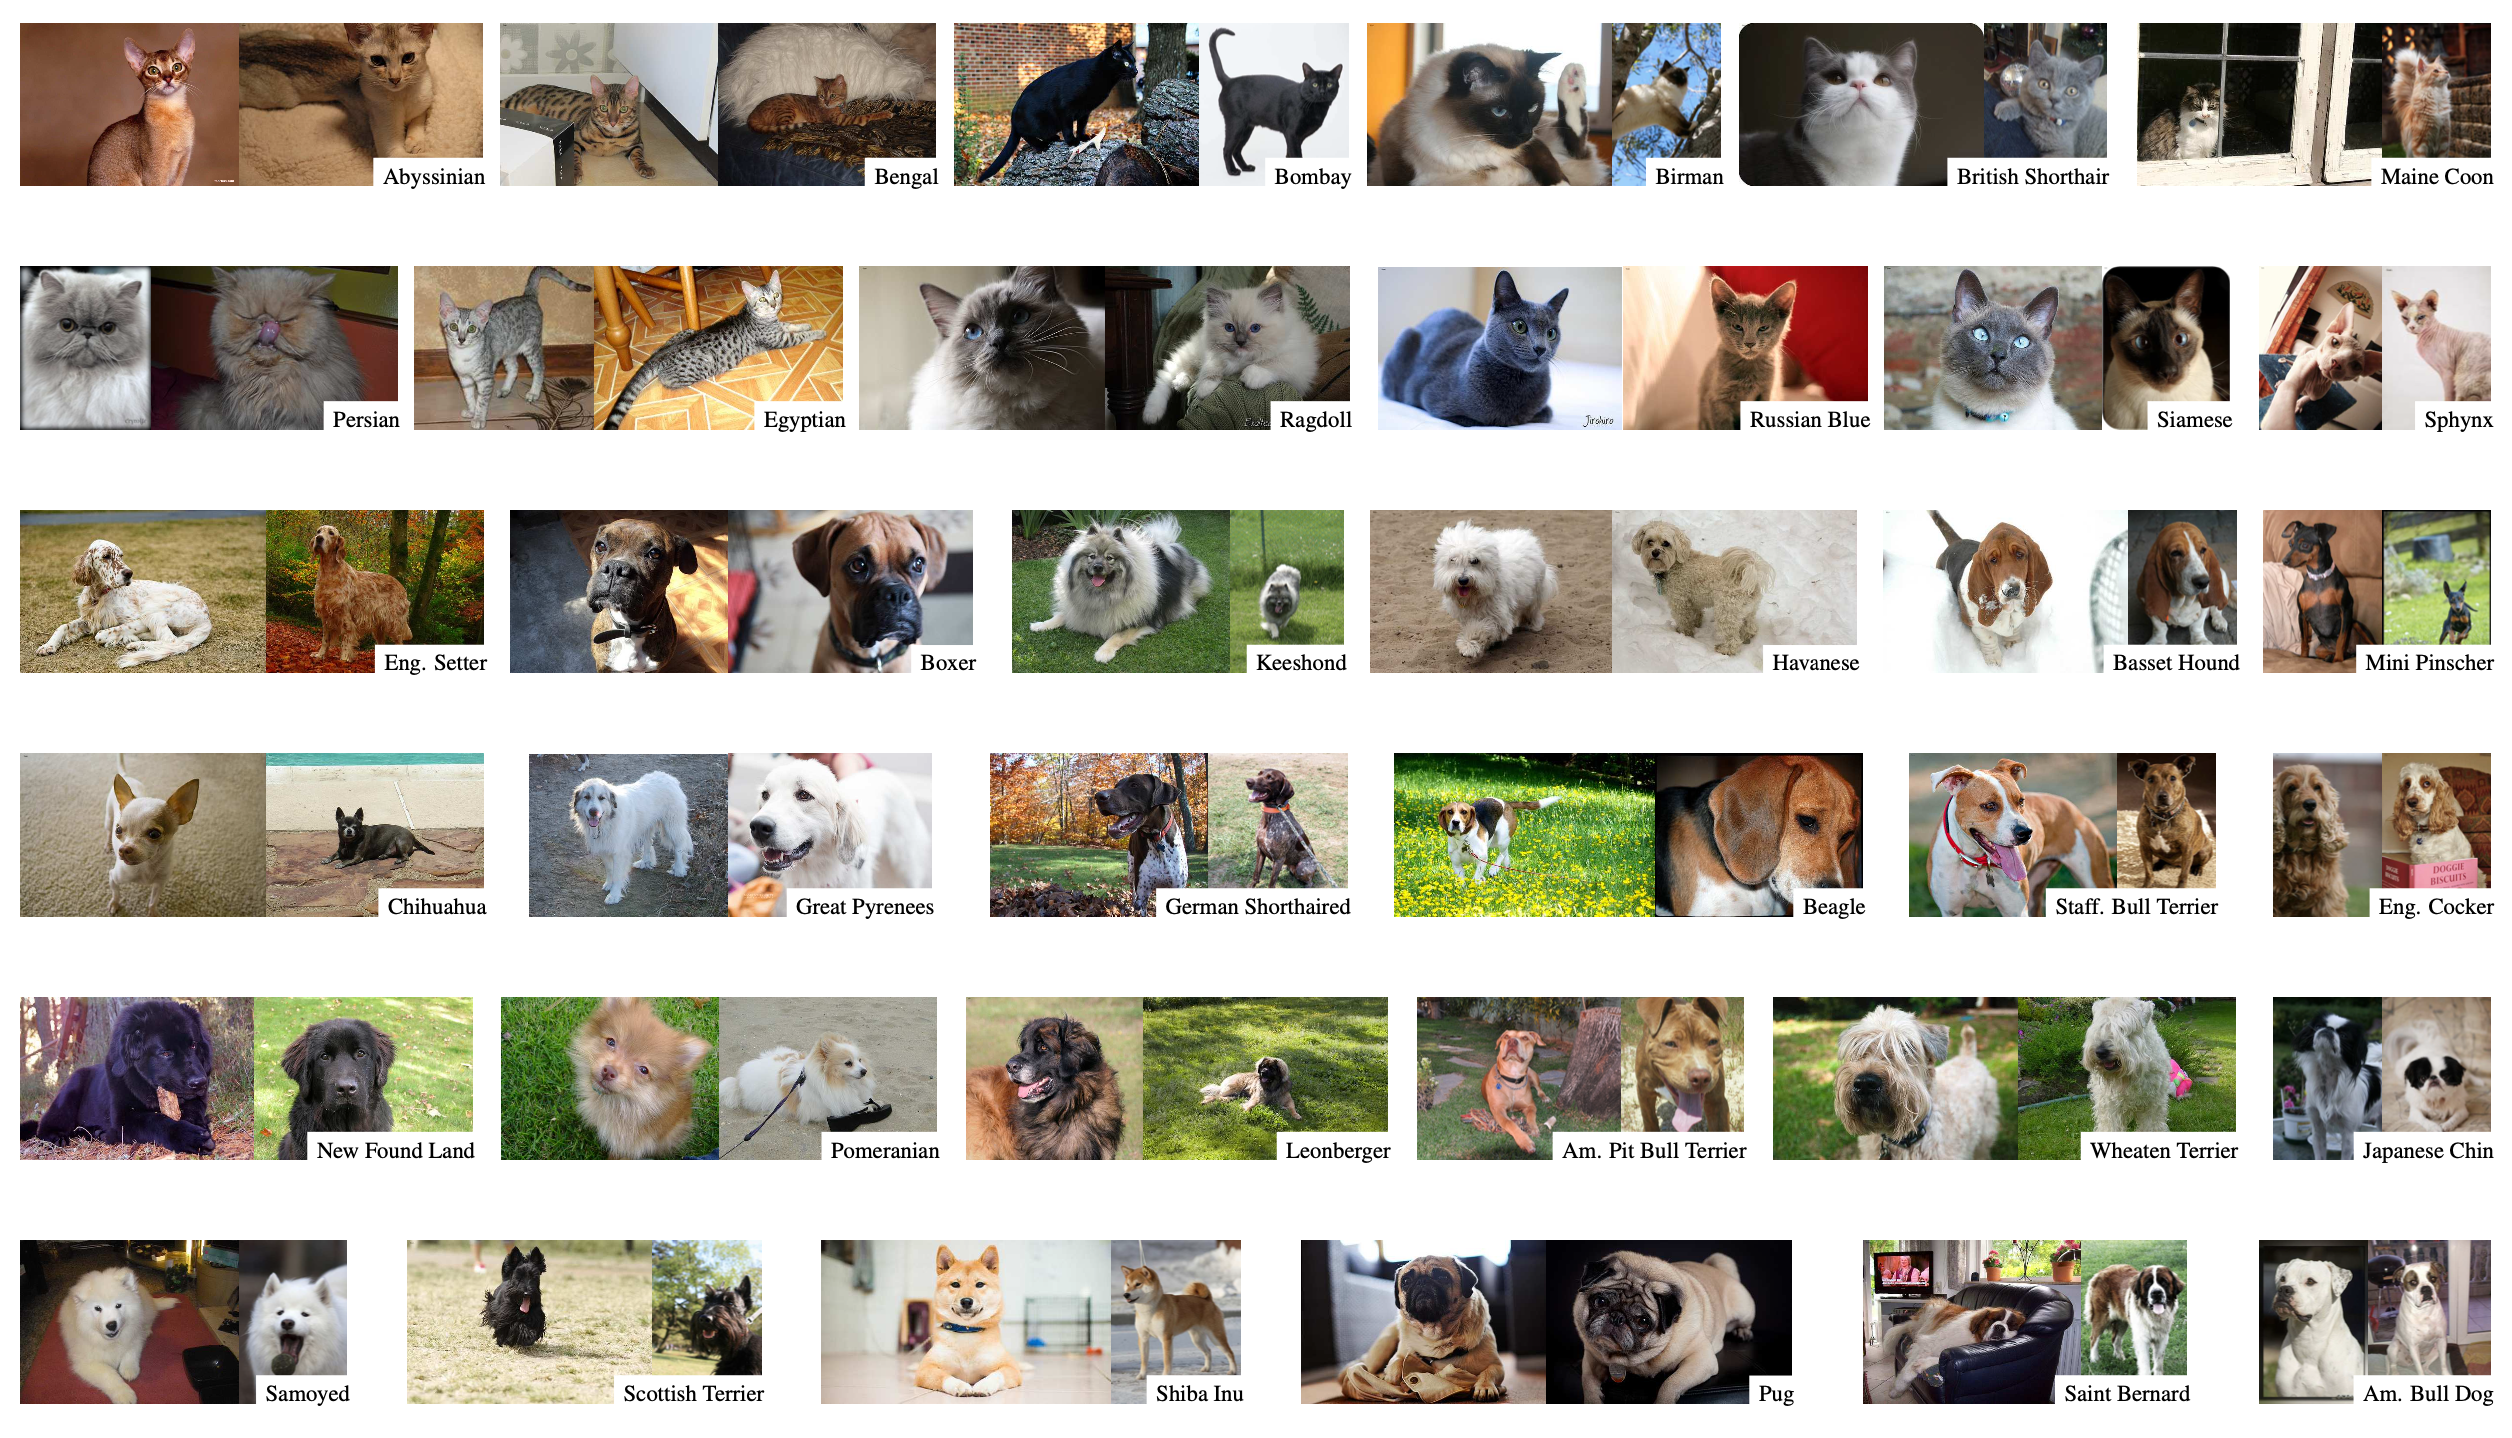
\includegraphics[width=1\textwidth]{Pictures/oxfordiiitPetC.png} 
    \caption{\textbf{Examples of each of the 37 Oxford-IIIT Pet classes} \cite{Parkhi2012CatsAD}. Note the significant variability found in the images, from changes in lighting and size to layout and scenery. This fact and the fact that it is a fine-grained dataset make it ideal for testing whether subject-driven augmentation is a competitive strategy.}
    \label{fig:oxfordiiitPetC}
\end{figure}

\begin{figure}
    \centering
    \includegraphics[width=1\textwidth]{Pictures/oxfordiiitPetS.png} 
    \caption{\textbf{Oxford-IIIT Pet annotations for segmentation}. Green is for the background region, yellow is for the ambiguous region, and purple is for the subject. }
    \label{fig:oxfordiiitPetS}
\end{figure}

We have chosen this dataset as the primary dataset for our analysis because it is fine-grained. This type of dataset contains many categories or classes with subtle distinctions between them. Unlike coarse-grained datasets with broader categories, fine-grained datasets focus on capturing fine details and subtle variations within a specific domain. Thus, given that the present work focuses on subject-driven augmentation techniques, such datasets allow us better discriminate the strengths and weaknesses of these techniques. In addition, the fact that this dataset contains both classification and segmentation annotations is also helpful.

On the other hand, the dataset used in experiment \textit{09-food-101} to show the versatility of the subject-driven augmentation technique is Food-101 \cite{bossard14}. This fine-grained dataset contains 101,000 images of 101 different food categories. We divide these images into 600 for training, 150 for validation and 250 for testing. It should be noted that both the training and validation images contain noise that the authors have not purposely cleaned to reflect that the real data is imperfect and contains large variability. Figure \ref{fig:food101} shows some images from this dataset showing the significant variability of the existing food types.

\begin{figure}
    \centering
    \includegraphics[width=1\textwidth]{Pictures/food101.png} 
    \caption{\textbf{Examples of 100 of the 101 Food-101 categories} \cite{bossard14}. Notice the significant variability of the existing food types and the fact that it is a fine-grained dataset.}
    \label{fig:food101}
\end{figure}